\section{Gate-Level Results (Part B)}\label{sec:gates}

\subsection{Method}\label{sec:gates:method}
The reference is the SPICE simulation of five static-CMOS gates (INV, NAND2, NOR2, AND2, OR2; AND2 and OR2 are simulated as complete gates, not as sums) for every input combination at the same 200 corners (18 cases $\times$ 200 $=$ 3,600 simulations), recording the leakage drawn from the supply $-i(V_{sup})$, the internal node voltages ($x$ between the series NMOS, $y$ between the series PMOS, and the first-stage output for AND2/OR2) and the output voltage.
% src: partB_gates/README.md, partB_gates/data/*.csv
Following step~4 of the project document, the terminal voltages $(V_d,V_g,V_s,V_b)$ of every transistor are taken from these \emph{recorded} SPICE node voltages (inputs at 0 or $V_{DD}$, NMOS bodies at 0, PMOS bodies at $V_{DD}$), together with the width and the corner's process parameters; the ML side does not solve the circuit. The ML internal-node columns of the prediction table are therefore copies of the recorded SPICE voltages. A transistor is ON if its gate is above $V_{DD}/2$ (NMOS) or below $V_{DD}/2$ (PMOS), and the model of that case predicts its four currents $\hat\imath_{m,t}$ (into terminal $t\in\{d,g,s,b\}$ of transistor $m$).
% src: ml/evaluate_gates.py, results/partB/gate_predictions.csv

\textbf{Gate leakage from the predicted currents.} The current drawn from $V_{DD}$ equals the sum of the currents into all terminals connected to the supply node, \emph{including} the nodes that an ON PMOS ties to it. Let $\mathcal S$ be the \emph{super-node}: $V_{DD}$ plus every node joined to $\mathcal S$ through the drain--source channel of an ON PMOS (iterated). With $n(m,t)$ the node of terminal $t$ of $m$ and $\mathcal M_{in}$ the transistors whose drain, source and body all lie in $\mathcal S$,
\begin{equation}
I_{leak}=\sum_{\substack{m\notin\mathcal M_{in}\\ t:\,n(m,t)\in\mathcal S}}\hat\imath_{m,t}\;+\sum_{\substack{m\in\mathcal M_{in}\\ n(m,g)\notin\mathcal S}}\bigl(-\hat\imath_{m,g}\bigr),
\label{eq:supernode}
\end{equation}
because for a transistor inside $\mathcal S$ Kirchhoff's law gives $i_d+i_s+i_b=-i_g$. The large channel current of an ON PMOS, which has almost no voltage across it, therefore cancels exactly and never has to be predicted (Fig.~\ref{fig:supernode}); what remains are OFF-transistor currents and gate currents.
\begin{figure}[t]
\centering
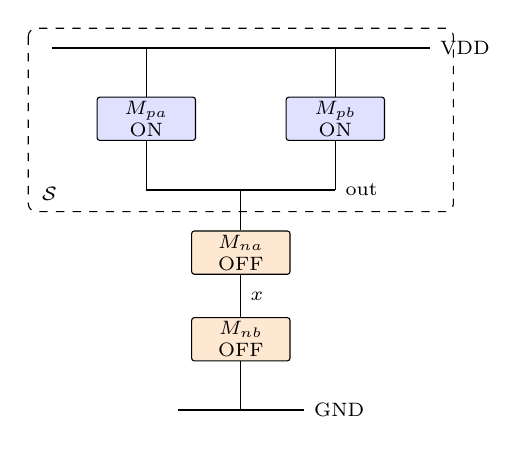
\begin{tikzpicture}[font=\scriptsize,
  tr/.style={draw,rounded corners=1pt,minimum width=1.25cm,minimum height=0.55cm,inner sep=1pt,align=center},
  on/.style={tr,fill=blue!12}, off/.style={tr,fill=orange!18}]
\draw[thick] (-2.4,2.7) -- (2.4,2.7) node[right]{VDD};
\node[on] (pa) at (-1.2,1.8) {$M_{pa}$\\ ON};
\node[on] (pb) at (1.2,1.8) {$M_{pb}$\\ ON};
\draw (pa.north) -- (-1.2,2.7); \draw (pb.north) -- (1.2,2.7);
\draw[thick] (-1.2,0.9) -- (1.2,0.9) node[right]{out};
\draw (pa.south) -- (-1.2,0.9); \draw (pb.south) -- (1.2,0.9);
\node[off] (na) at (0,0.1) {$M_{na}$\\ OFF};
\node[off] (nb) at (0,-1.0) {$M_{nb}$\\ OFF};
\draw (0,0.9) -- (na.north); \draw (na.south) -- (nb.north) node[midway,right]{$x$};
\draw[thick] (-0.8,-1.9) -- (0.8,-1.9) node[right]{GND}; \draw (nb.south) -- (0,-1.9);
\draw[dashed,rounded corners=3pt] (-2.7,2.95) rectangle (2.7,0.62);
\node[anchor=south west] at (-2.65,0.64) {$\mathcal S$};
\end{tikzpicture}
\caption{Super-node $\mathcal S$ (dashed) for a NAND2 with inputs 00. Both PMOS are ON, so $V_{DD}$ and the output form one node. The leakage of (\ref{eq:supernode}) is the current $\hat\imath_d$ of the OFF transistor $M_{na}$ leaving $\mathcal S$ plus $-\hat\imath_g$ of the two PMOS, whose drain, source and body all lie in $\mathcal S$; their channel currents cancel.}
\label{fig:supernode}
\end{figure}

\textbf{Metrics.} For every simulation $i$ the error is $e_i=(\hat I_i-I_i)/I_i$ with the ML leakage $\hat I_i$ and the SPICE leakage $I_i$; the bias is the median of $e_i$; a group is a gate case. The project document states a target of ``up to 99\,\% mean accuracy'' without defining it, so we use $A_1=1-\overline{|e|}$ as the headline and report three alternatives in Sec.~\ref{sec:assumptions}.

\subsection{Results}\label{sec:gates:results}
Over all 3,600 gate simulations the mean accuracy is 98.87\,\% (median 99.18\,\%, 95th percentile of $|e|$ 3.24\,\%, maximum 8.10\,\%); 35 rows exceed 5\,\% and 1,529 exceed 1\,\%. Per gate the mean accuracy is 98.47\,\% (INV), 99.02\,\% (NAND2), 98.96\,\% (NOR2), 98.84\,\% (AND2) and 98.85\,\% (OR2). The 18-case table is Table~\ref{tab:gate}, the parity plot Fig.~\ref{fig:gateparity}.
\textbf{The 99\,\% target is not reached at gate level:} 98.87\,\% is 0.13 points short. The most accurate cases are NAND2 \texttt{00} (99.49\,\%), NOR2 \texttt{11} (99.46\,\%) and NAND2 \texttt{10} (99.44\,\%); the least accurate are INV with input 0 (98.37\,\%), NOR2 \texttt{00} (98.38\,\%) and OR2 \texttt{11} (98.39\,\%). The latter three all contain an NMOS OFF transistor with the full supply across it; Sec.~\ref{sec:errors} traces the error to that operating point. The biases are small (between $-0.73$ and $+1.17\,\%$).
% src: results/partB/gate_predictions.csv, results/partB/gate_results.csv, results/analysis/report_numbers/error_breakdown.txt
\begin{table*}[t]
\caption{Gate results (final model set): SPICE and ML median leakage, bias (median signed error), median and 95th-percentile $|e|$, and mean accuracy $A_1$ for the 18 gate cases (200 corners each).}
\label{tab:gate}
\centering\footnotesize
% src: results/partB/gate_results.csv
\begin{tabular}{llrrrrrr}
\toprule
Gate & Inputs & SPICE med. (A) & ML med. (A) & Bias (\%) & Med. err. (\%) & P95 err. (\%) & Mean acc. (\%) \\
\midrule
INV & 0 & \num{2.19e-08} & \num{2.21e-08} & -0.73 & 1.24 & 4.35 & 98.37 \\
INV & 1 & \num{9.82e-08} & \num{9.81e-08} & +1.17 & 1.20 & 3.50 & 98.58 \\
\midrule
NAND2 & 00 & \num{5.40e-10} & \num{5.37e-10} & -0.03 & 0.39 & 1.29 & 99.49 \\
NAND2 & 01 & \num{5.00e-08} & \num{5.03e-08} & -0.13 & 1.09 & 4.29 & 98.57 \\
NAND2 & 10 & \num{8.53e-09} & \num{8.54e-09} & -0.08 & 0.34 & 1.83 & 99.44 \\
NAND2 & 11 & \num{1.95e-07} & \num{1.95e-07} & +1.14 & 1.19 & 3.48 & 98.59 \\
\midrule
NOR2 & 00 & \num{4.38e-08} & \num{4.42e-08} & -0.73 & 1.24 & 4.34 & 98.38 \\
NOR2 & 01 & \num{2.04e-07} & \num{2.02e-07} & +0.69 & 0.96 & 3.50 & 98.79 \\
NOR2 & 10 & \num{1.61e-08} & \num{1.61e-08} & +0.44 & 0.64 & 1.98 & 99.23 \\
NOR2 & 11 & \num{2.26e-10} & \num{2.28e-10} & -0.12 & 0.42 & 1.42 & 99.46 \\
\midrule
AND2 & 00 & \num{9.92e-08} & \num{9.98e-08} & +1.16 & 1.19 & 3.48 & 98.59 \\
AND2 & 01 & \num{1.67e-07} & \num{1.66e-07} & +0.06 & 0.82 & 2.74 & 99.05 \\
AND2 & 10 & \num{1.13e-07} & \num{1.14e-07} & +0.80 & 0.91 & 3.27 & 98.77 \\
AND2 & 11 & \num{2.26e-07} & \num{2.30e-07} & +0.46 & 0.78 & 2.88 & 98.95 \\
\midrule
OR2 & 00 & \num{1.60e-07} & \num{1.61e-07} & +0.03 & 0.80 & 2.74 & 99.01 \\
OR2 & 01 & \num{2.38e-07} & \num{2.41e-07} & +0.08 & 0.81 & 2.88 & 98.99 \\
OR2 & 10 & \num{4.31e-08} & \num{4.22e-08} & -0.39 & 0.74 & 2.75 & 99.02 \\
OR2 & 11 & \num{2.22e-08} & \num{2.23e-08} & -0.72 & 1.20 & 4.34 & 98.39 \\
\bottomrule
\end{tabular}

\end{table*}
\begin{figure}[t]
\centering
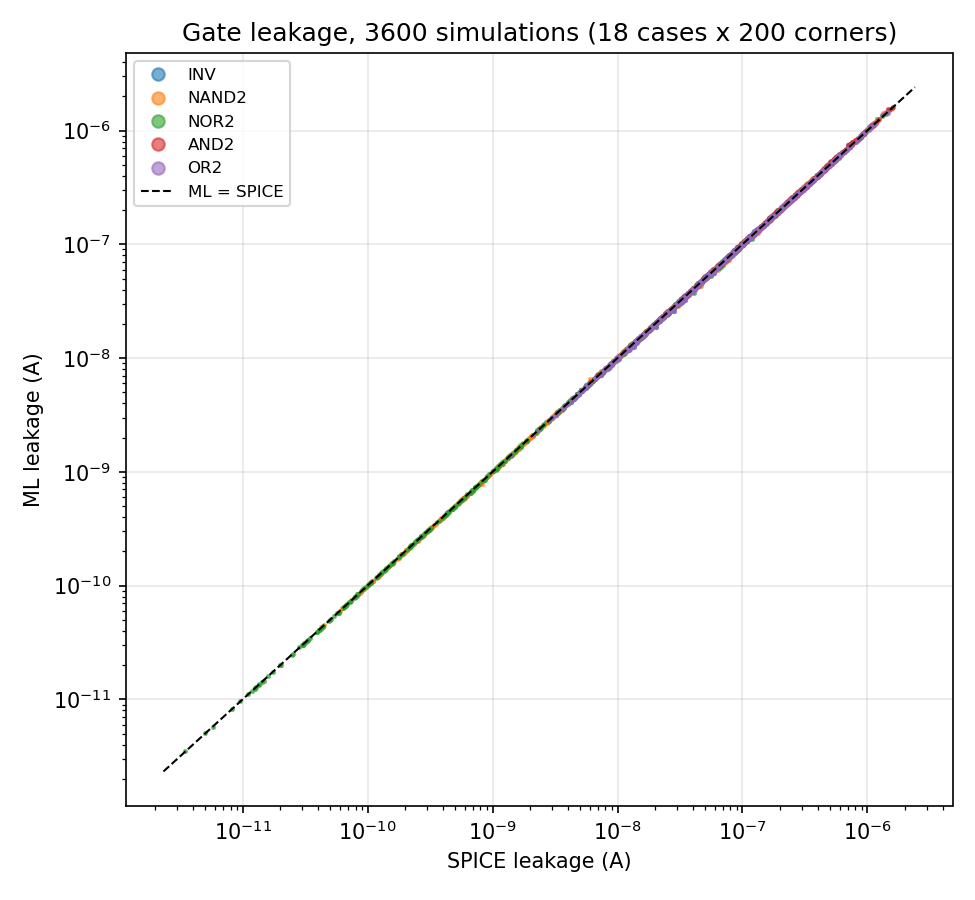
\includegraphics[width=\columnwidth]{figures/gate_parity.png}
\caption{ML versus SPICE leakage for all 3,600 gate simulations (log axes, dashed line: ML $=$ SPICE). The points follow the diagonal over about five decades; the deviations are at the percent level (maximum 8.10\,\%).}
\label{fig:gateparity}
% src: results/partB/gate_parity.png
\end{figure}

\subsection{Why the plain current sum fails}\label{sec:gates:plain}
The literal reading of ``use the predicted currents to calculate the gate leakage'' is the sum of the predicted currents into the terminals tied to the $V_{DD}$ node. This fails by orders of magnitude (Table~\ref{tab:plainsum}): NAND2 and AND2 reach a mean accuracy of $-5.7\times10^{5}\,\%$ and $-2.2\times10^{3}\,\%$ with 265 rows of negative predicted leakage, and over all gates the mean accuracy is of the order of $-10^{5}\,\%$. The reason is the one of Sec.~\ref{sec:data:corners}: an ON PMOS inside a gate has almost no voltage across it, so its channel current is the small difference of two large numbers that the models cannot resolve, whereas (\ref{eq:supernode}) cancels it exactly.
\textbf{Check with exact currents.} We re-simulated 10 rows of every one of the 18 gate cases with a 0\,V source in series with every transistor terminal and fed the \emph{exact SPICE} terminal currents to (\ref{eq:supernode}) (same code as the ML evaluation, same ON/OFF rule): over 179 converged simulations the result reproduces the recorded leakage to $\num{8.0e-6}$ relative at worst (median $\num{6.5e-7}$), which is the six-digit CSV precision. The construction is therefore exact; all remaining gate error is model error.
% src: results/analysis/report_numbers/plain_sum_check.csv, validation_checks/c1_kcl_method.csv, c1_kcl_method.txt
\begin{table}[t]
\caption{Plain sum of the currents into the $V_{DD}$ terminals versus the super-node method (final models, 3,600 rows).}
\label{tab:plainsum}
\centering\footnotesize
\setlength{\tabcolsep}{2.5pt}
\fitcol{% src: results/analysis/report_numbers/plain_sum_check.csv
\begin{tabular}{lrrrrr}
\toprule
Gate & Plain sum: mean acc. (\%) & Neg. rows & Med. err. (\%) & Super-node: mean acc. (\%) & Med. err. (\%) \\
\midrule
INV & 16.7 & 0 & 3.43 & 98.47 & 1.23 \\
NAND2 & -567,002 & 137 & 41.13 & 99.02 & 0.58 \\
NOR2 & 56.1 & 0 & 1.74 & 98.96 & 0.74 \\
AND2 & -2,167 & 128 & 11.49 & 98.84 & 0.91 \\
OR2 & 24 & 0 & 23.00 & 98.85 & 0.86 \\
\midrule
All gates & -126,462 & 265 & 12.97 & 98.87 & 0.82 \\
\bottomrule
\end{tabular}
}
\end{table}
